\chapter{Clustering in Feature Space}\label{chapter:clustering_in_feature_space}

In this chapter, we introduce the pipeline we intend to use for performing unsupervised image segmentation. We focus on retrieving the different clusters found in the feature space of a pretrained CNN. The intuition is that CNN models have shown great performance in classification and related reasoning tasks, which is attributed to the fact that the models have learned rich high-level feature representations. These representations do not only encode local pixel information, but also semantic information which in the context of real world images is related to the different objects found in the image and how they are positioned relative to each other. Thus, an approach based on clustering these features is likely going to consider a high-level representation of the objects in the image. The outline of our approach is shown in \autoref{fig:outline}.
\begin{figure}[thbp]
    \centering
    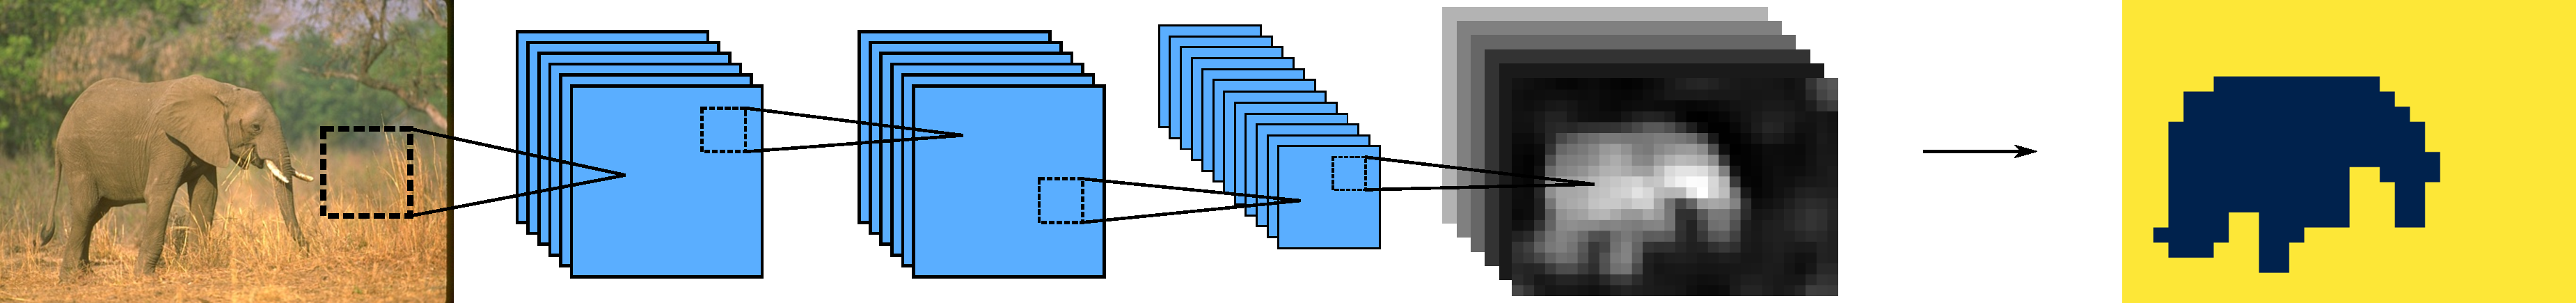
\includegraphics[width=\linewidth]{figures/outline.pdf}
    \caption{An overview of our pipeline to extract different objects in an image. First, the image is passed down the feature extractor of a pretrained CNN. Then, similar pixels of the resulting feature image are clustered together to yield the final segmentation mask.}
    \label{fig:outline}
\end{figure}

\section{Feature Extraction}

In this section, we transform an input color image into a tensor of features. The tensor of features can be thought of as a multi-channel image which we call the feature image. Each channel, or \emph{feature map}, in the feature image can capture some regional semantic information. In our work, we explore extracting the feature image from the VGG16 network \parencite{simonyan2014very} (shown in \autoref{fig:vgg16}). The CNN has performed remarkably well in the classification task of the ImageNet Large-Scale Visual Recognition Challenge in 2014.

The architecture of VGG16 is made up of a feature extractor and a classifier. The feature extractor is characterized by its block structure and its repeated downsampling layers, which are responsible for reducing the spatial resolution of the input tensor in order to extract significant semantic information. The classifier is made up of three dense layers followed by a softmax activation layer. The final output tensor represents a list of class probability scores that can be used to classify the input image.

Since our task is to generate a high-dimensional feature representation of the input image and not to classify it, we will focus on the feature extractor part of the network. Also, this allows us to input images of arbitrary spatial resolutions to the network without being constrained by the classifier's fixed input size. Therefore, unless otherwise stated, we refer to the feature extractor part of the network directly using the network's name.

\begin{figure}[t]
    \centering
    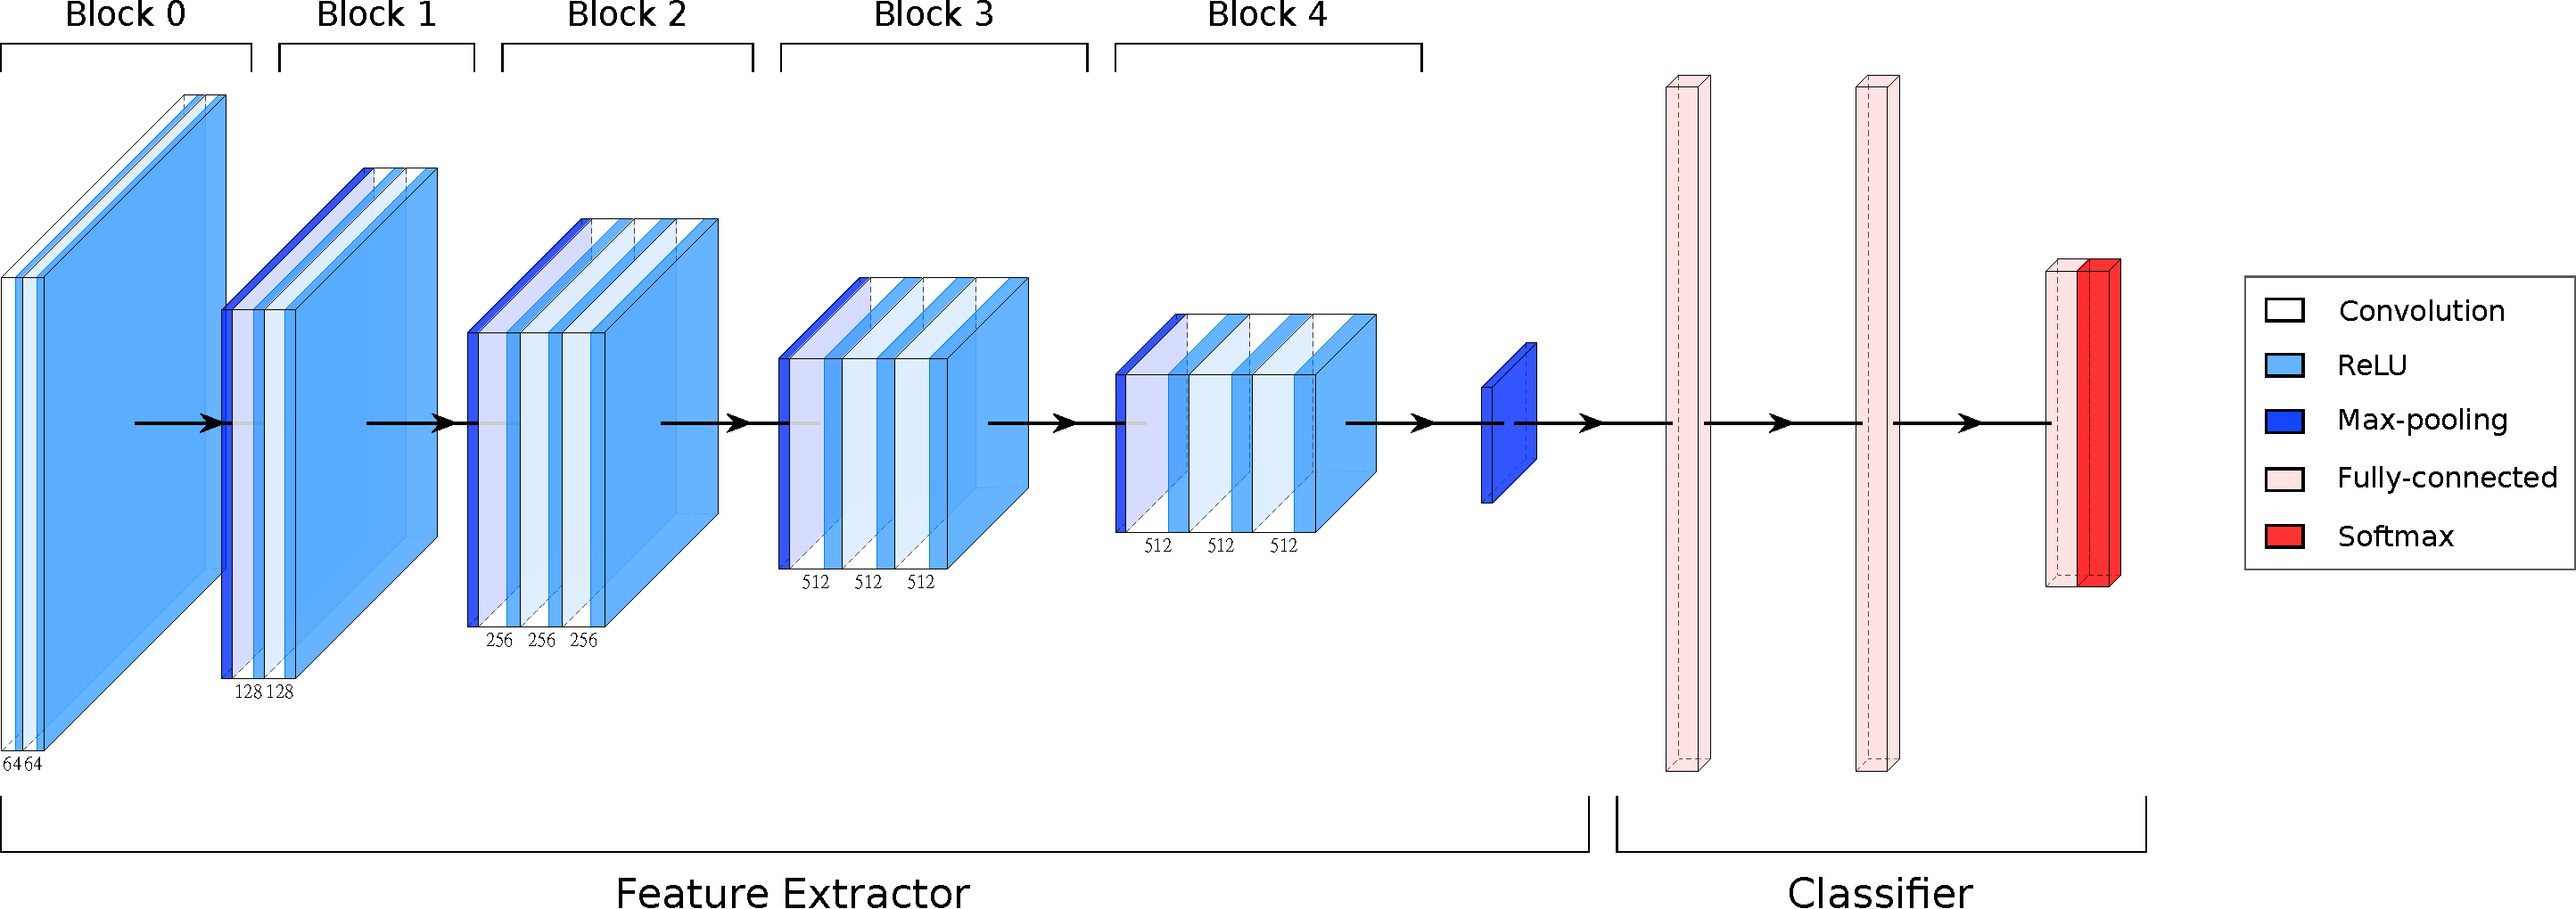
\includegraphics[width=\textwidth]{figures/vgg16.pdf}
    \caption[Caption for LOF]{A schematic representation showing the architecture of VGG16\footnotemark. The number below each layer refers to the number of feature maps in the layer's output tensor.}
    \label{fig:vgg16}
\end{figure}

After obtaining the feature image, a segmentation mask is created by clustering the feature pixels and labelling each pixel by its cluster membership. However, due to the high dimensionality of the pixels in the feature image, this approach might not yield satisfactory results. Points in a high-dimensional dataset are often very sparse. The data is said to suffer from the \emph{curse of dimensionality} \parencite{bishop2006pattern}.

\section{Dimension Reduction}

\footnotetext{Figure was generated using \url{https://github.com/HarisIqbal88/PlotNeuralNet}}

In order to alleviate the curse of dimensionality, the feature pixels need to be further processed. \emph{Principal Component Analysis} (PCA) \parencite{wold1987principal} is a well-known dimensionality reduction technique which can be used to re-express a given set of points with a new coordinate system. The method returns a new set of basis vectors (principal components) ranked by the variance of the data along the vectors. The least variance-capturing principal components are often truncated, thereby reducing the dimensionality of the data while still capturing most of its variance.

More formally, let $X \in \mathbb{R}^{m \times n}$ represent an $m$-dimensional mean-centered dataset consisting of $n$ data points. PCA tries to find a new representation of $X$ such that:
\begin{equation}
    Y = PX
\end{equation}
where $P \in \mathbb{R}^{d \times m}$ is the new basis matrix and $Y \in \mathbb{R}^{d \times n}$ is the new set of projected points in $d$-dimensional space. The goal of PCA is to reduce the redundancy of the new representation of $X$. This is achieved by making the new data matrix decorrelated. In other words, the covariance matrix of $Y$ should be a diagonal matrix with zeros in the off-diagonal elements \parencite{shlens2014tutorial}:
%% PROOF
\begin{align*}
    C_Y &= \frac{1}{n}YY^T
    = \frac{1}{n}(PX)(PX)^T
    = PC_XP^T
    = P(E^TDE)P^T
    = D.
\end{align*}
By setting the projection matrix $P$ equal to the matrix of eigenvectors $E$, a new decorrelated representation of the data matrix $X$ can be obtained. Additionally, the diagonal elements of $C_Y$ contain the eigenvalues which represent the variance of the data along the respective principal component.

After obtaining the new representation of the feature image, the principal components with the lowest eigenvalues are truncated. In our work, the number of depth dimensions in the feature image is reduced to the minimum number of principal components required to capture 99\% of the variance in the data.

\begin{figure}[t]
    \centering
    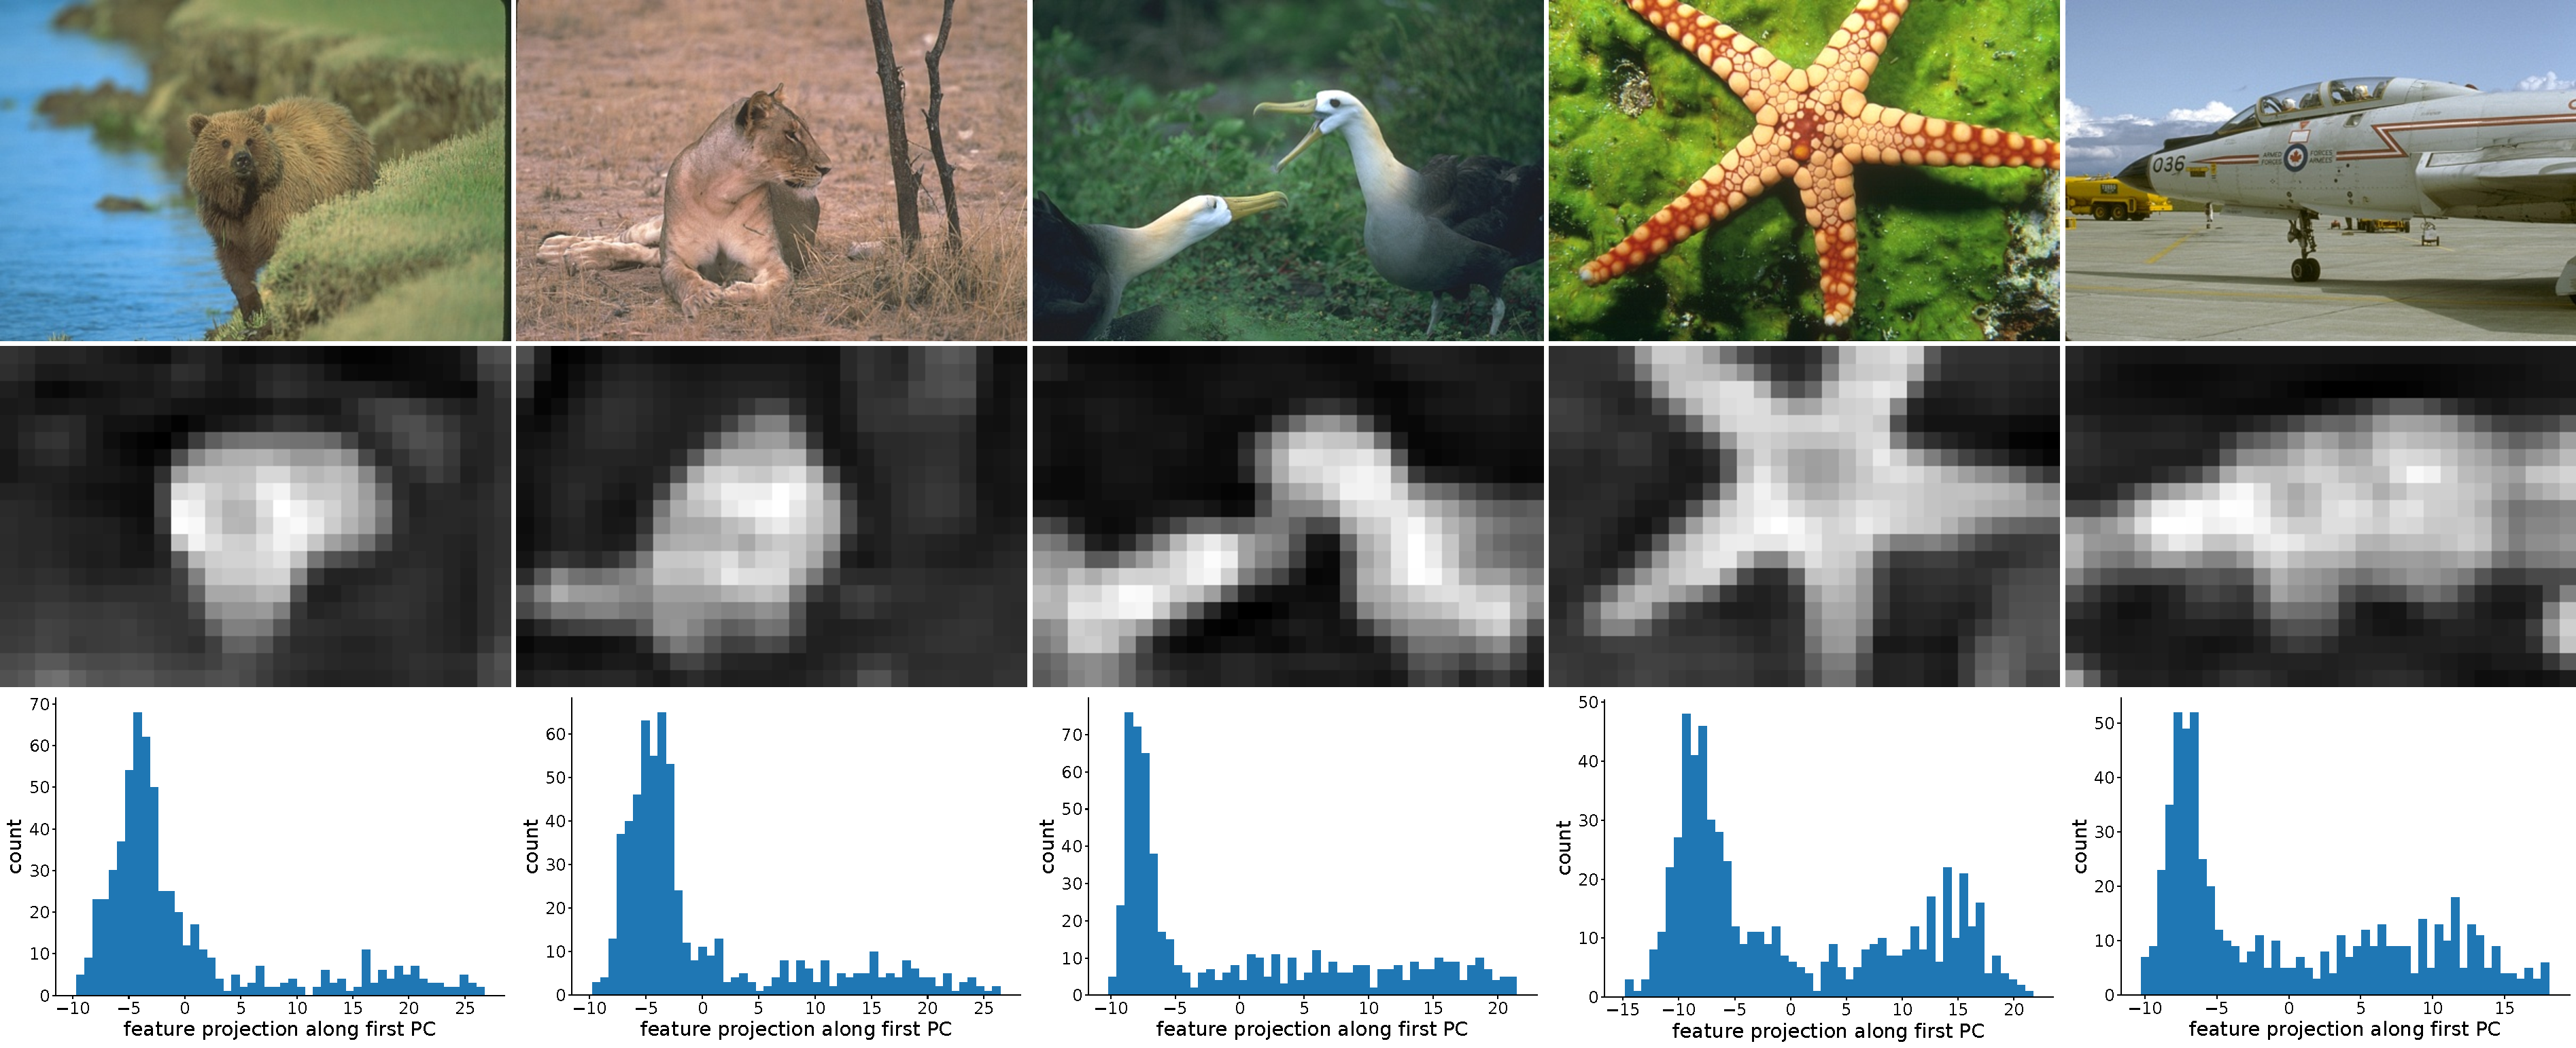
\includegraphics[width=\textwidth]{figures/first_pc.pdf}
    \caption{Five images (top row) and the projections of their extracted features along the first principal component (middle row), where greater values are represented by brighter pixels. The histograms of the projections (bottom row) are used to visualize the distribution of the features along the first principal component.}
    \label{fig:first_pc}
\end{figure}
\autoref{fig:first_pc} shows five images and the projections of their feature images along the first principal component. The figure shows that the foreground and the background are separated in some images, which is further supported by the two peaks shown in most of the histograms.

\section{Clustering Similar Pixels}

After reducing the dimensionality of the feature image, it can be segmented using the methods discussed in the previous chapter. We investigate segmenting the feature image (of reduced dimensionality) using two methods:
\begin{itemize}
    \item The first method applies the superpixel-based segmentation approach introduced in \autoref{subsection:color_based_segmentation} to the feature image. First, FSLIC is applied to generate a segmentation of the feature image into feature superpixels. Next, similar superpixels are clustered together using SFCM to yield the final segmentation result. This approach is relatively fast and does not suffer from pixel-level feature variation that might mislead the subsequent clustering step.
    \item The second method investigates clustering the feature pixels directly using k-means. Compared to the first method, this method has the advantage of having less hyperparameters. In addition, feature pixels cover smaller regions with respect to the original image compared to feature superpixels (see \autoref{fig:receptive_fields}). Hence, feature pixels are able to summarize a smaller number of objects in comparison to feature superpixels.
\end{itemize}

\begin{figure}[!h]
    \centering
    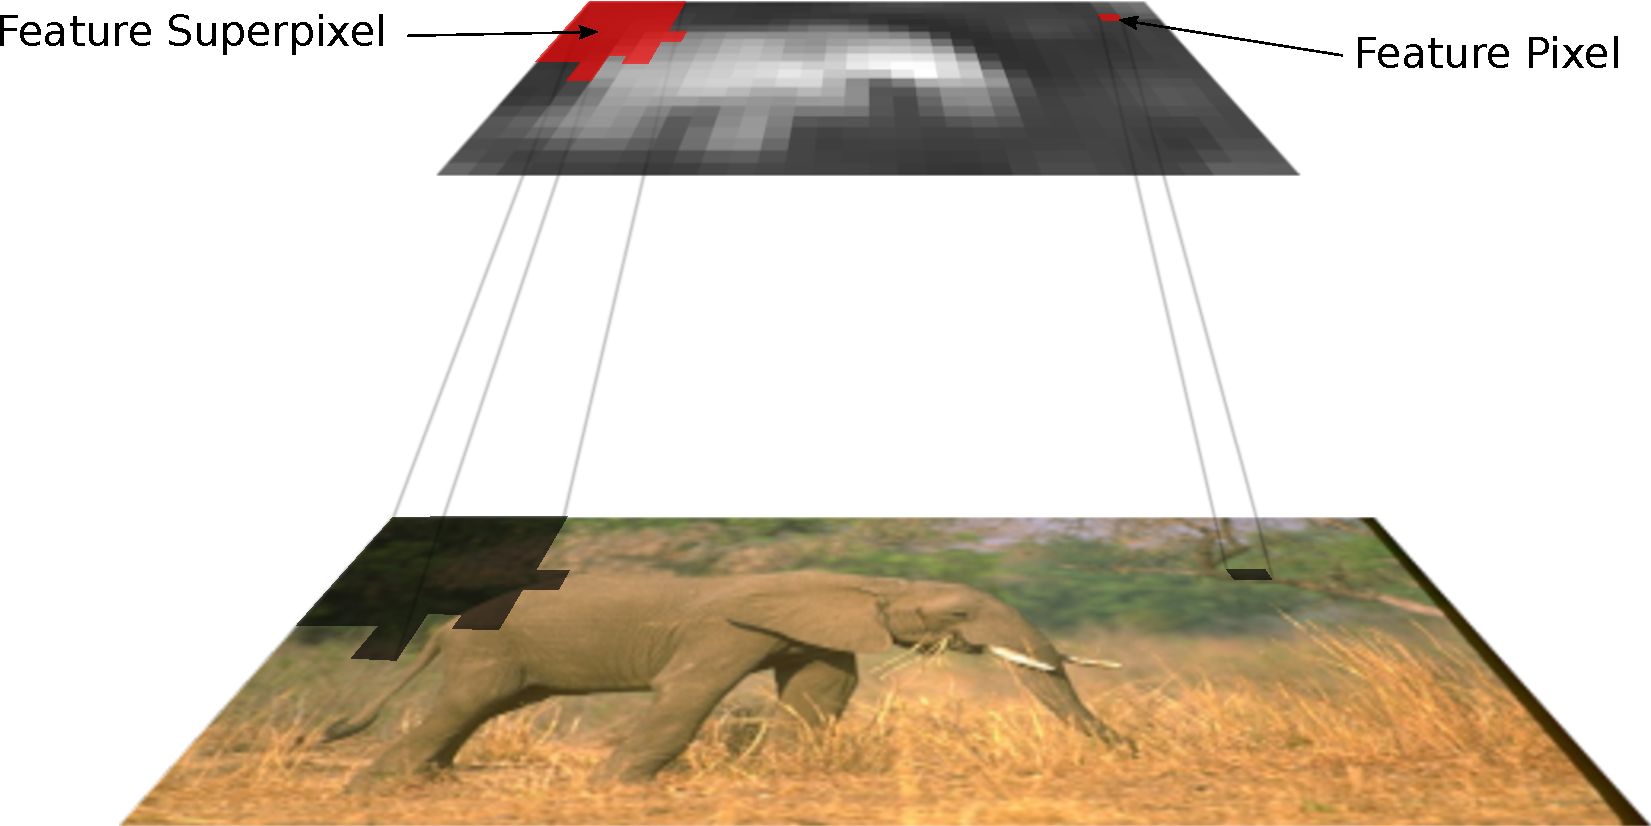
\includegraphics[width=.65\textwidth]{figures/receptive_fields.pdf}
    \caption{A feature pixel covers a smaller region with respect to the original image compared to a feature superpixel.}
    \label{fig:receptive_fields}
\end{figure}

The clustering algorithms used in both methods (SFCM and k-means) are parameterized by the cluster number $k$. In our work, we choose $k$ according to the silhouette method (see \autoref{subsection:k-means_limitations}). The value of $k_{\text{max}}$ (the upper limit of the cluster number search interval) should not be too large to avoid yielding an over-segmented result. In our experiments in \autoref{chapter:experiments_and_results}, we choose $k_{\text{max}}$ based on the size and content of the image. Furthermore, since both algorithms are sensitive to the initial cluster center positions, they are run multiple times and the clustering result with the lowest within cluster distances is taken to be the final result.